% Slides for 2025-01-27
% To create a slide, use the following:
% \begin{frame}{TITLE}
%     BODY
% \end{frame}

% To create a slide with a bullet list, use the following:
\begin{frame}{Potting Update}
    \begin{itemize}
        \item Added wax to screw imprints and airways
        \item Hollow in the fin plug, even though we had covered the airways and the resin had nearly overflowed
    \end{itemize}    
\end{frame}

\begin{frame}{Images}
    \centering
    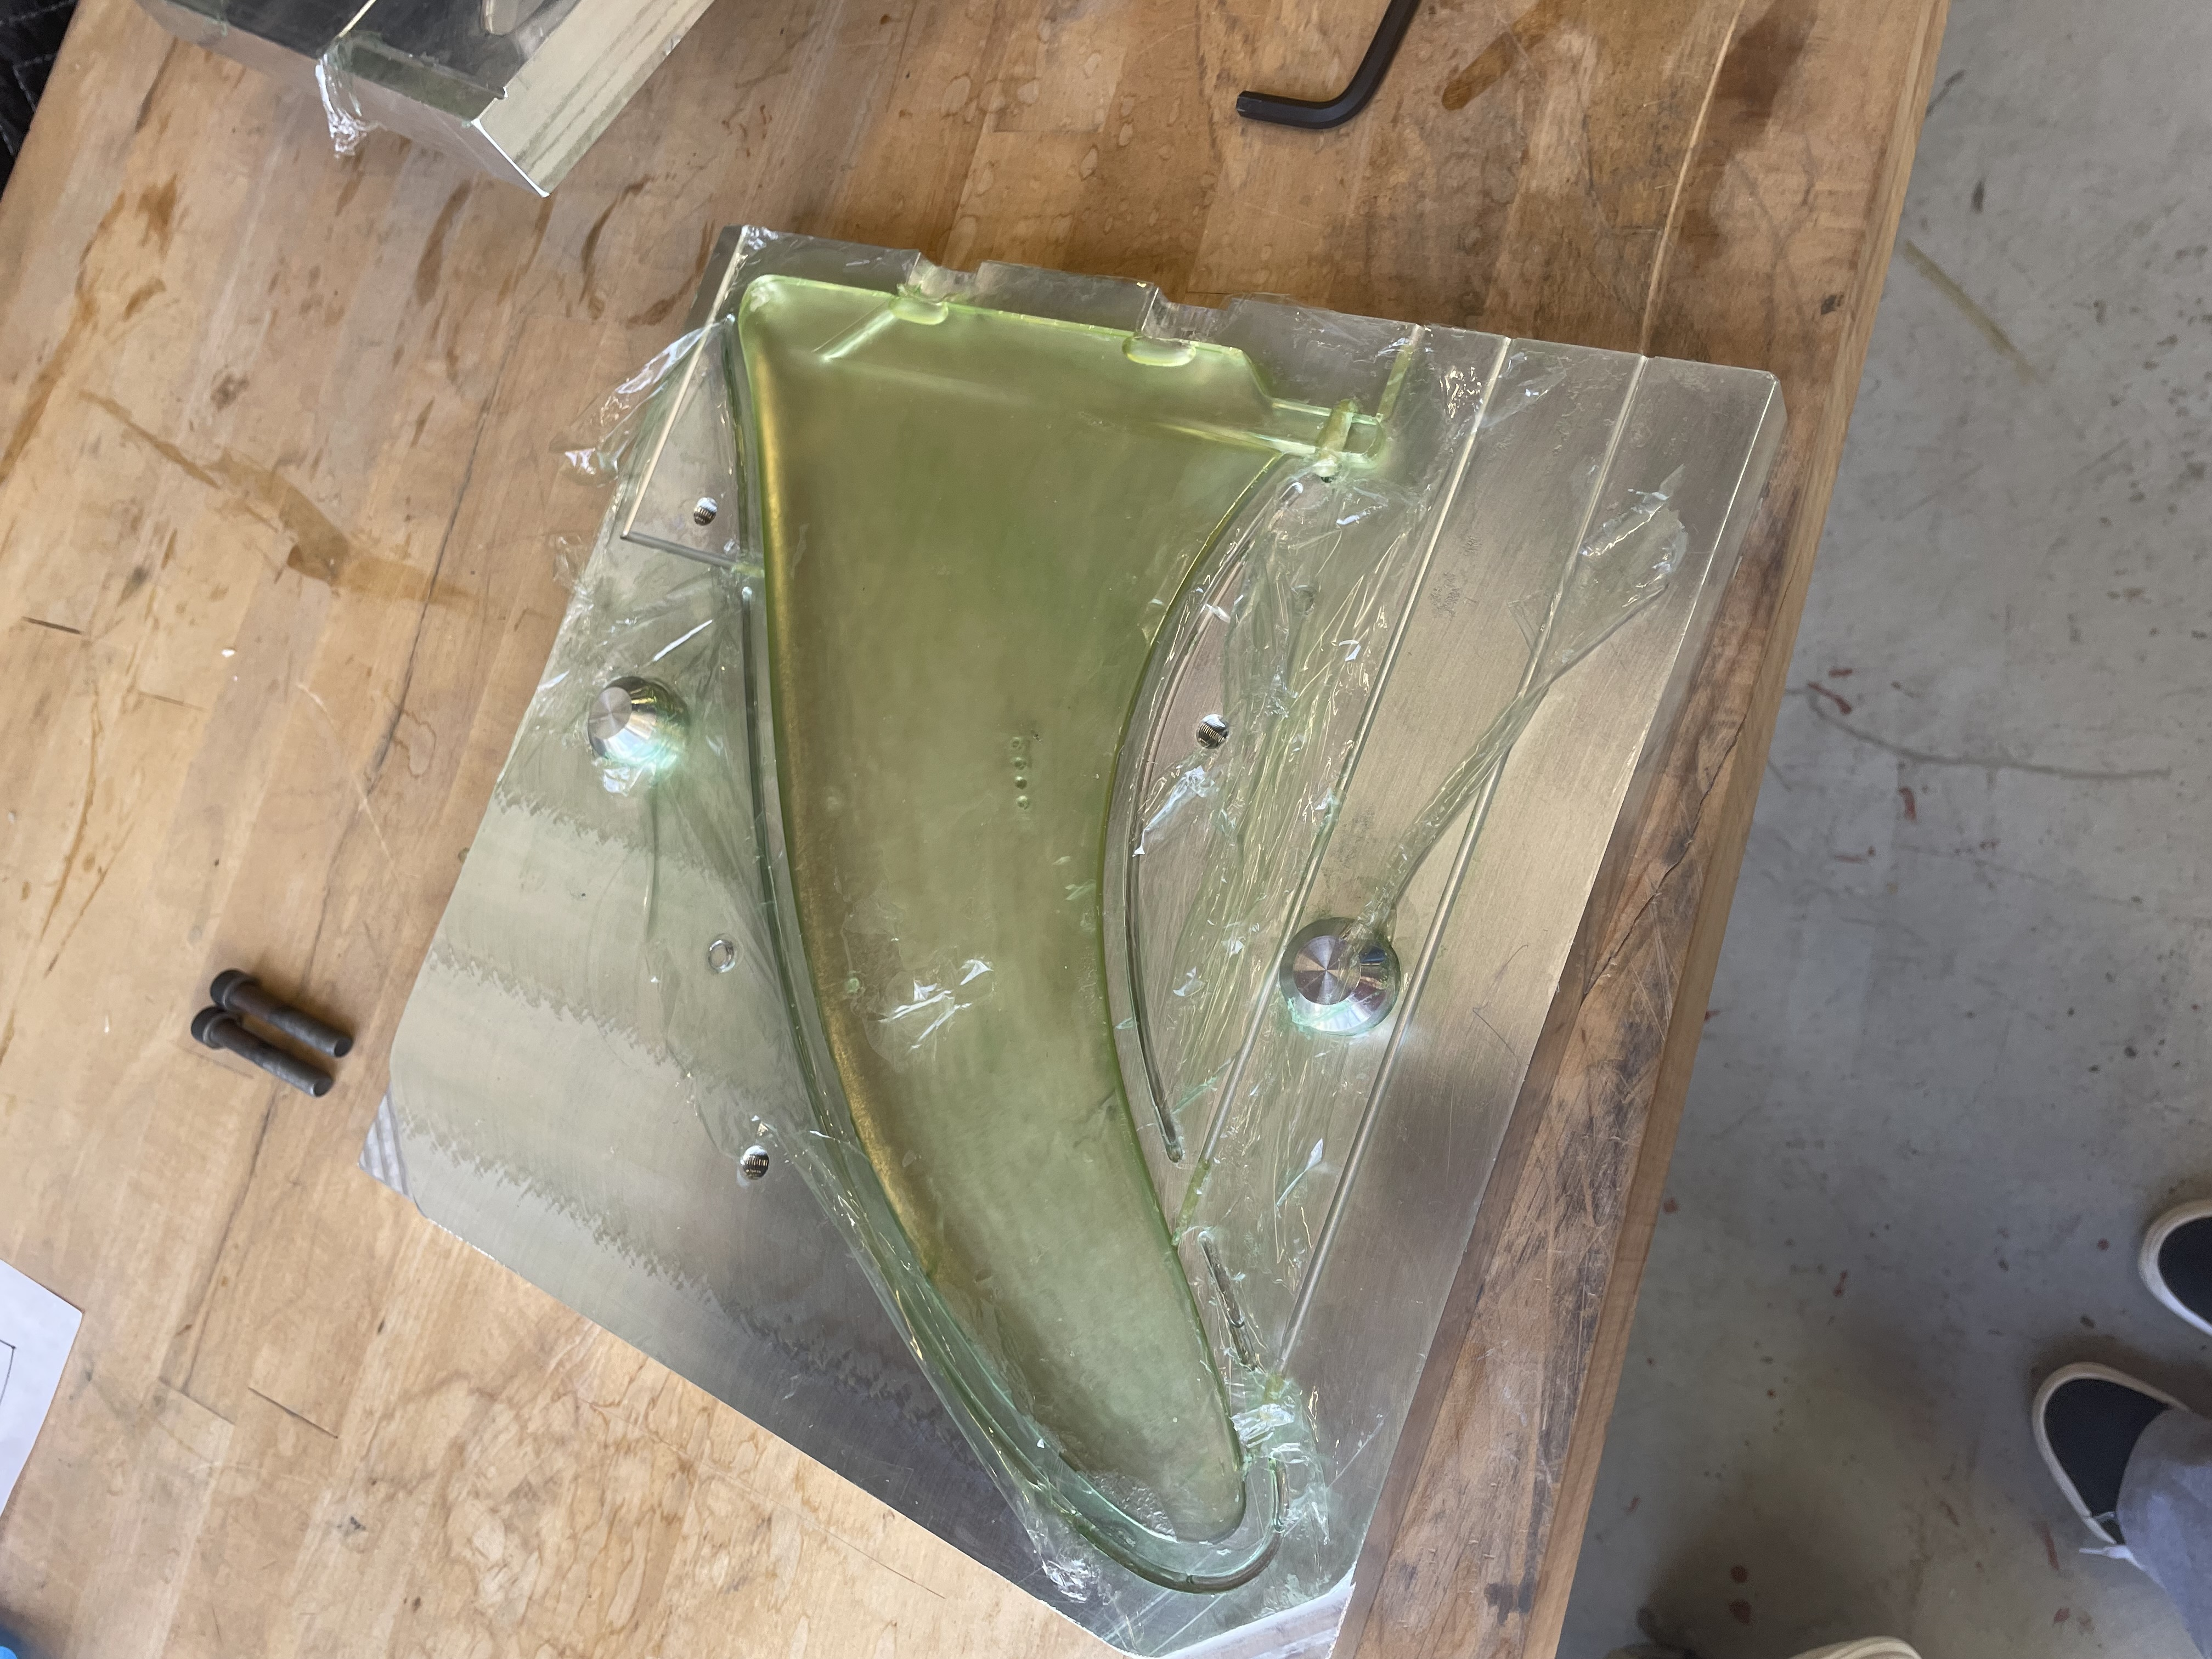
\includegraphics[height=0.45\textheight,width=0.45\textwidth,keepaspectratio]{images/sf_img_7573.jpg}
    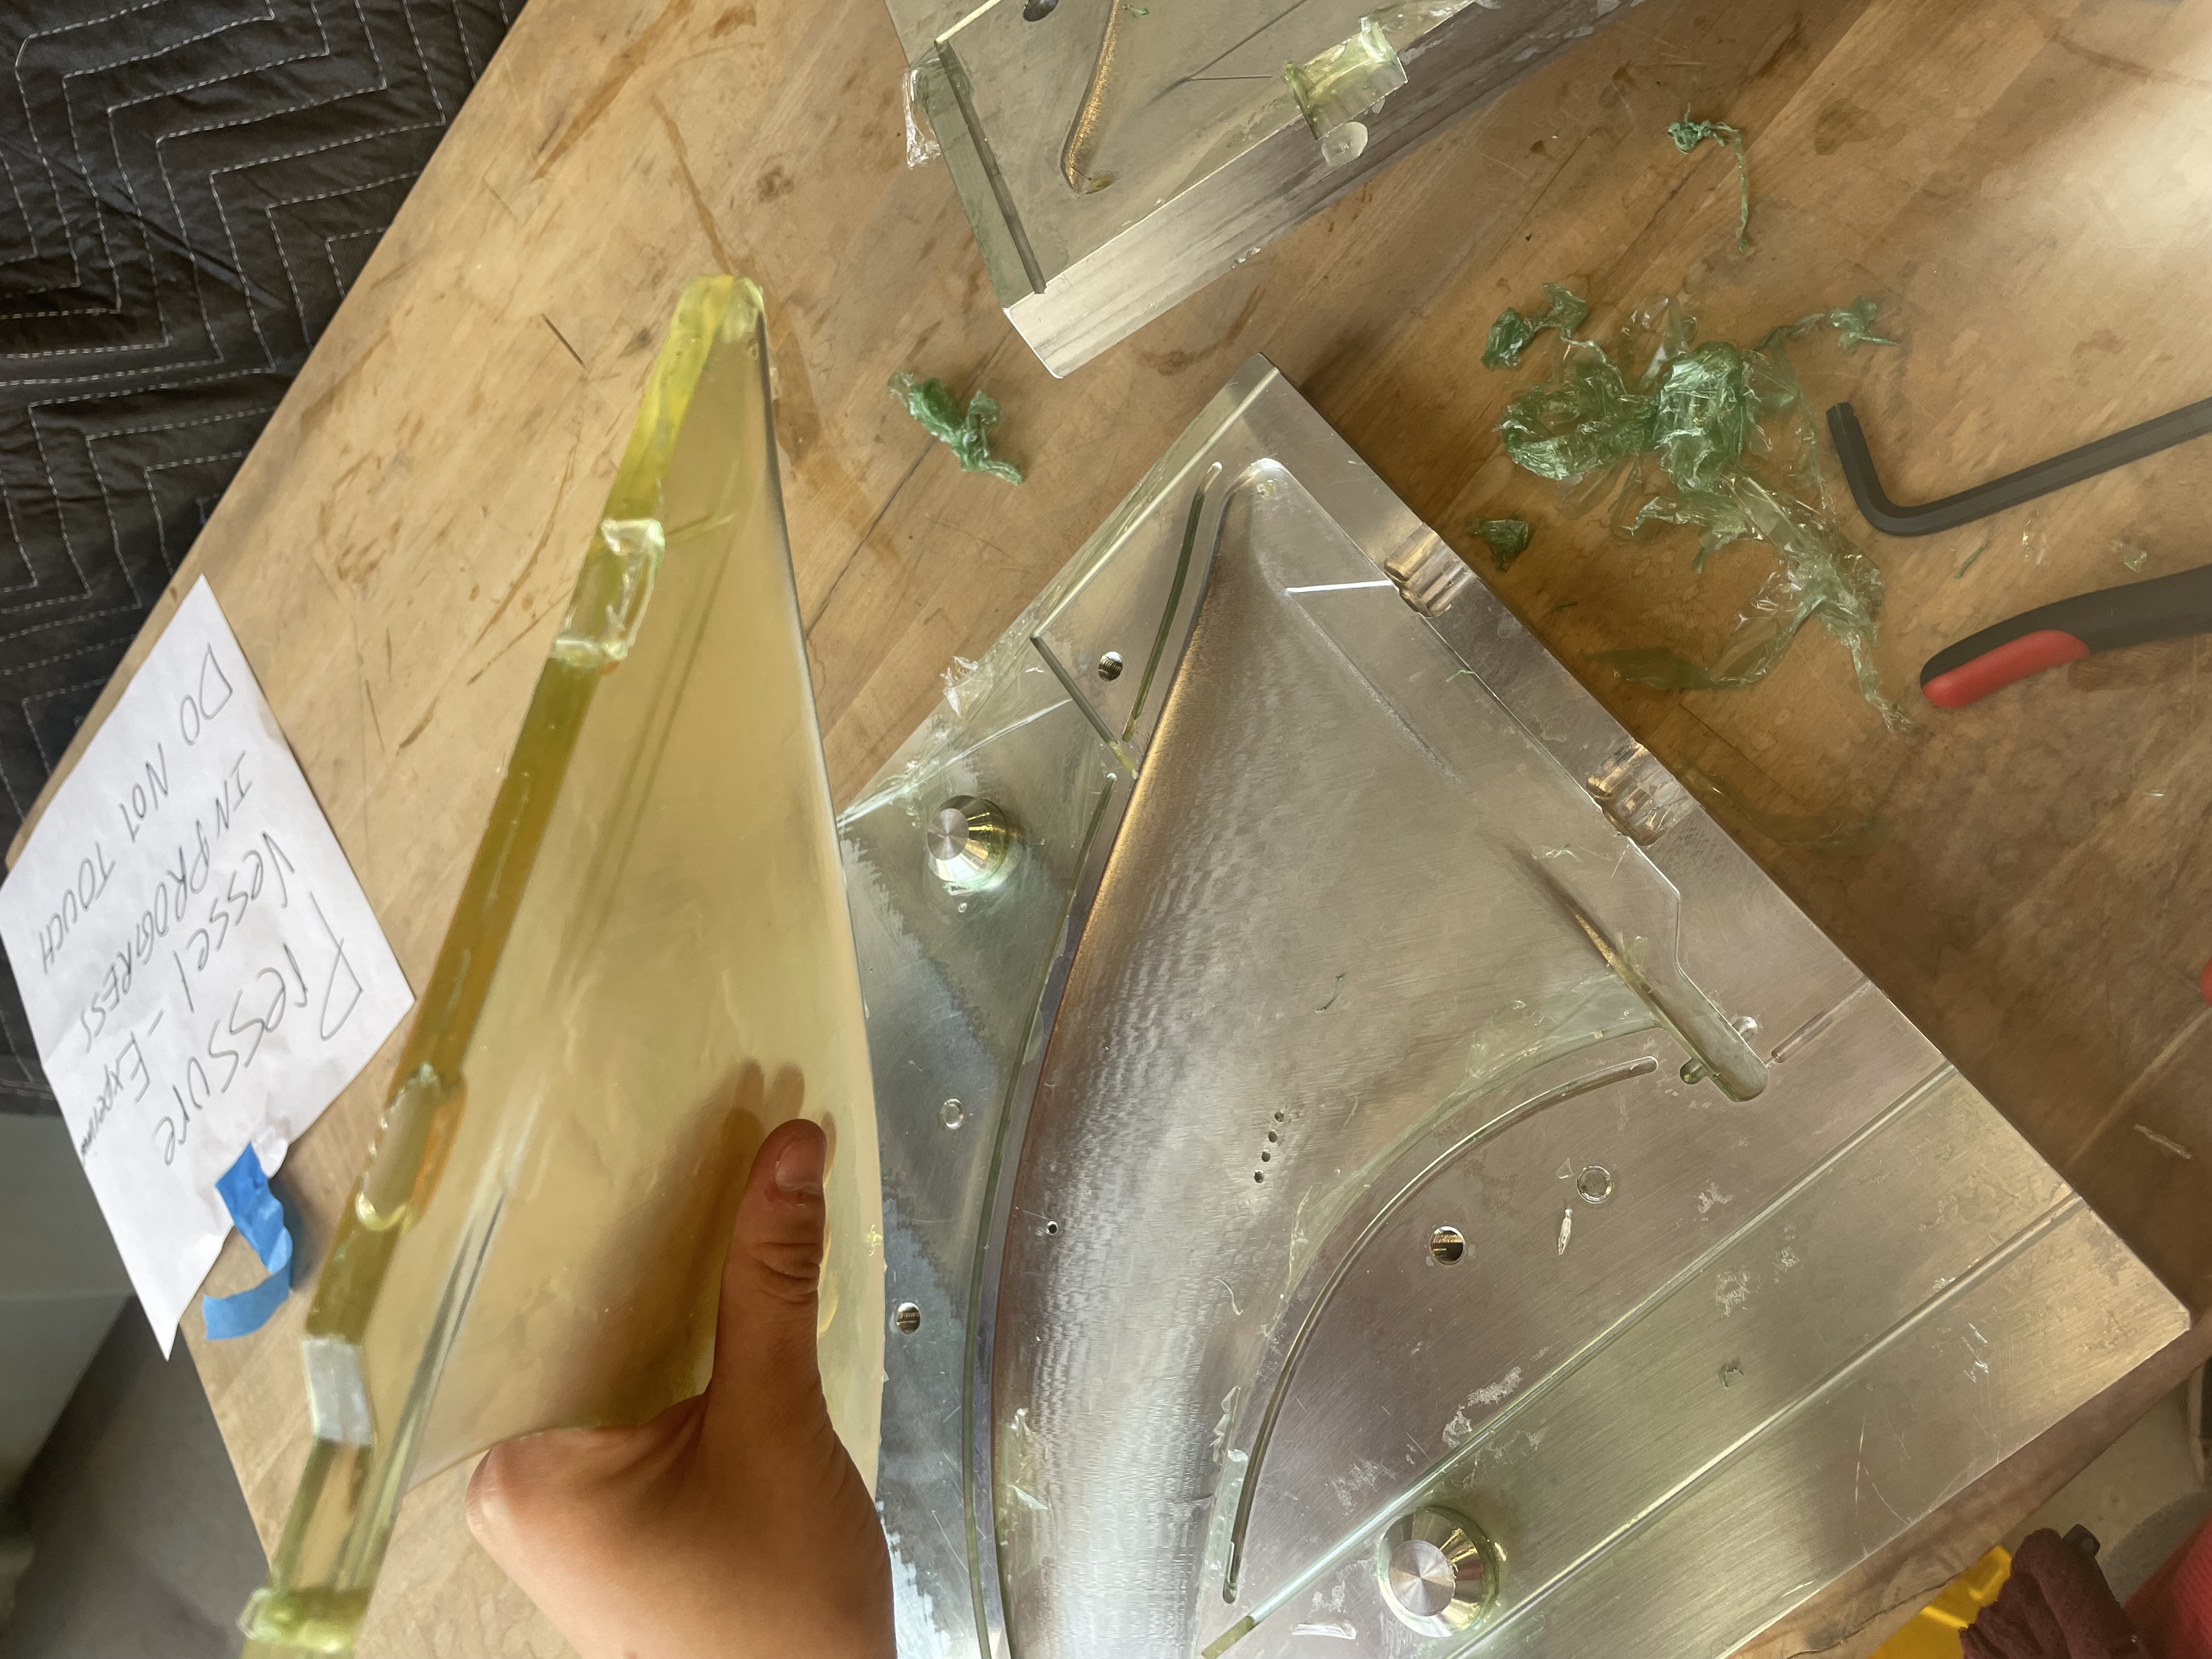
\includegraphics[height=0.45\textheight,width=0.45\textwidth,keepaspectratio]{images/sf_img_7575.jpg}
    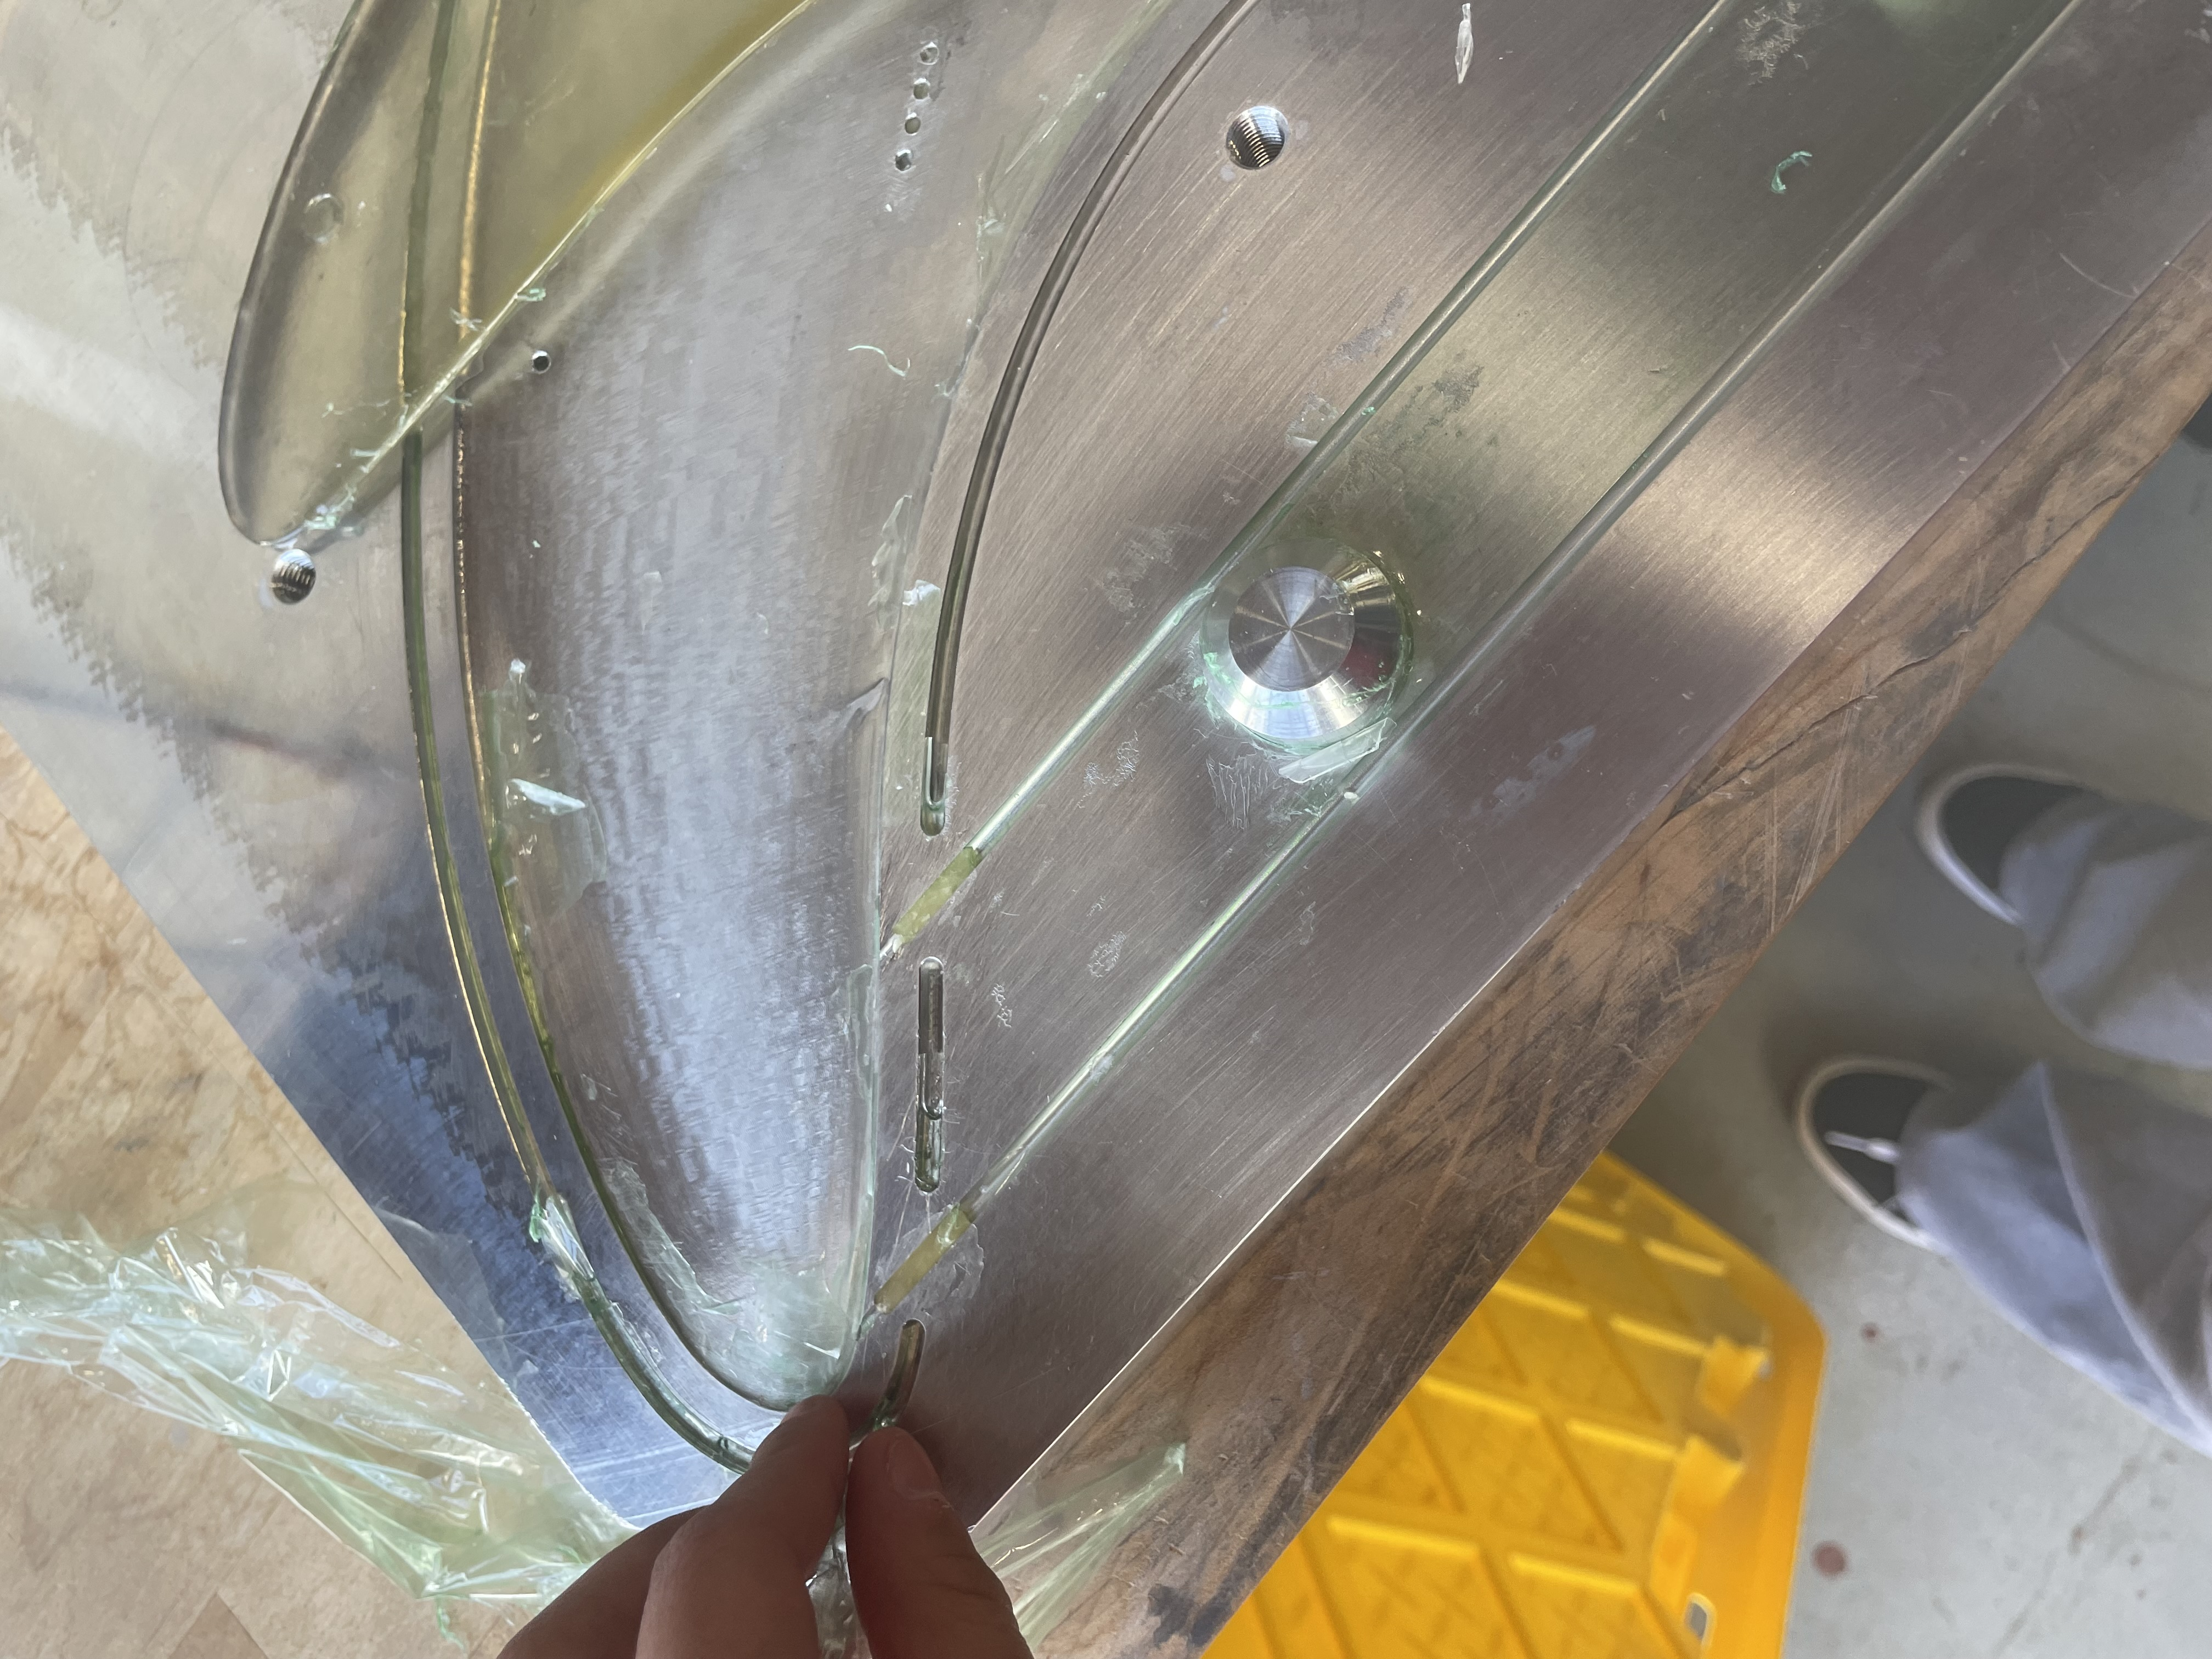
\includegraphics[height=0.45\textheight,width=0.45\textwidth,keepaspectratio]{images/sf_img_7576.jpg}
    
\includegraphics[height=0.45\textheight,width=0.45\textwidth,keepaspectratio]{images/sf_img_7577.jpg}
\end{frame}

\begin{frame}{Project Status}
    \centering
    
\includegraphics[height=0.9\textheight,width=0.9\textwidth,keepaspectratio]{images/sf_project_status.png}
\end{frame}
% To create a slide with numbered list, use the following:
% \begin{frame}{TITLE}
%     \begin{enumerate}
%         \item ITEM 1
%         \item ITEM 2
%     \end{enumerate}
% \end{frame}

% To create a slide with a graphic:
% 1. Add the graphic to this folder (named picture.png)
% 2. Use the following:
% \begin{frame}{TITLE}
%     \centering
%     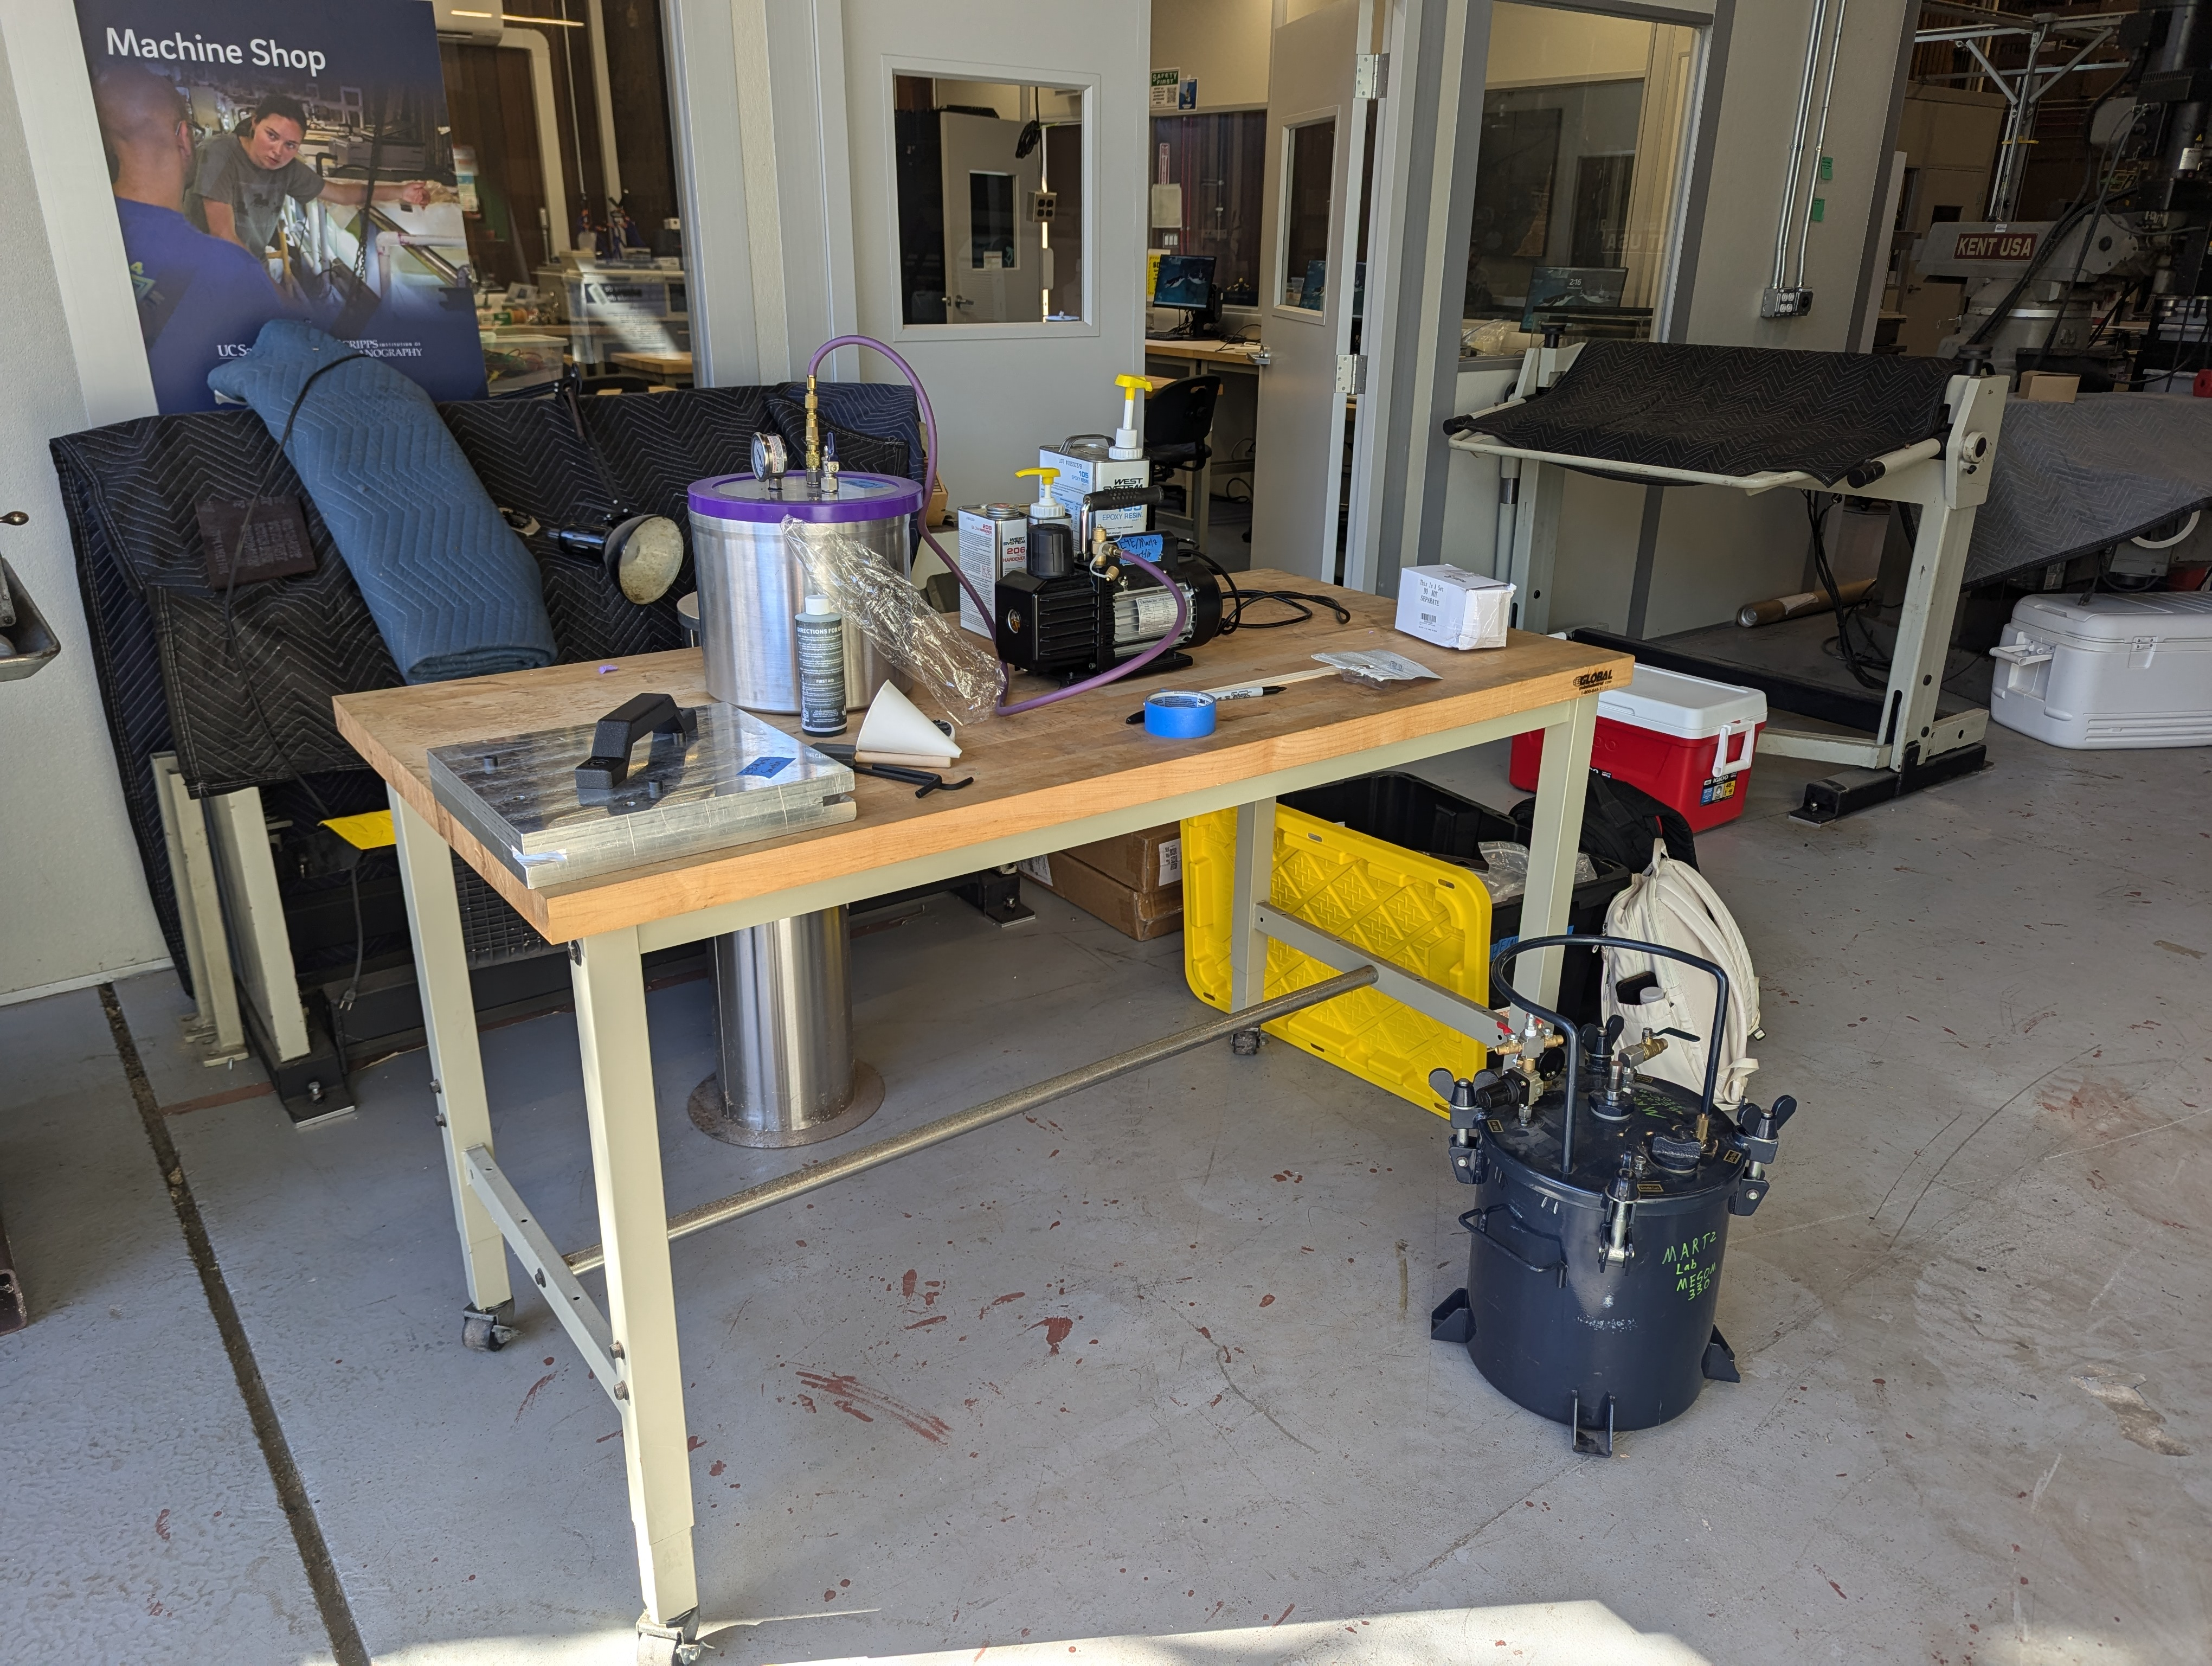
\includegraphics[height=0.7\textheight,width=0.7\textwidth,keepaspectratio]{images/sf_potting_setup.jpg}
% \end{frame}

% To create a slide with two columns, use the following:
% \begin{frame}{TITLE}
%     \begin{columns}
%         \begin{column}{0.5\textwidth}
%             COLUMN 1 BODY
%         \end{column}
%         \begin{column}{0.5\textwidth}
%             COLUMN 2 BODY
%         \end{column}
%     \end{columns}
% \end{frame}
